\section{Programm Strukturen}
% TODO: Besser Lösung als Raisebox finden um die Bilder zu zentrieren.
\begin{tabular}{ll}
	\hline
	\textbf{if L then S} & \textbf{if L then S1 else S2} \\
  	\raisebox{0.55cm}{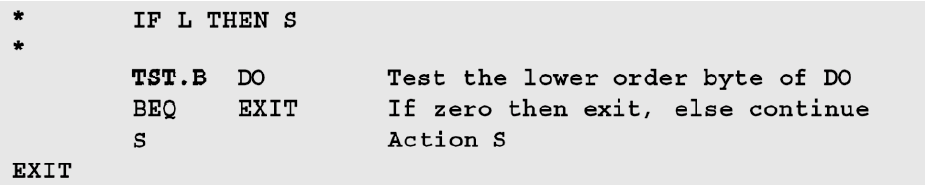
\includegraphics[width=9cm]{images/IfThen.PNG}} & 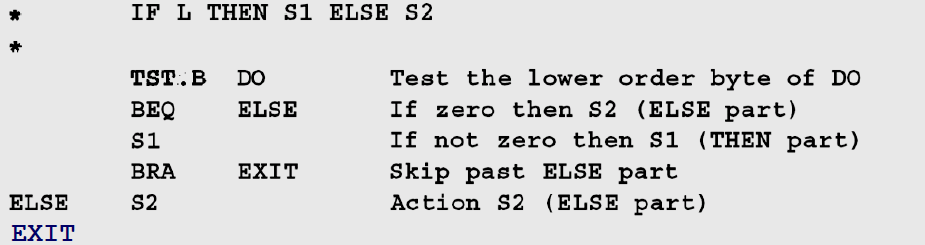
\includegraphics[width=9cm]{images/IfThenElse.PNG} \\
	\hline
	\textbf{for I=n1 to n2 do} & \textbf{while L do S} \\
  	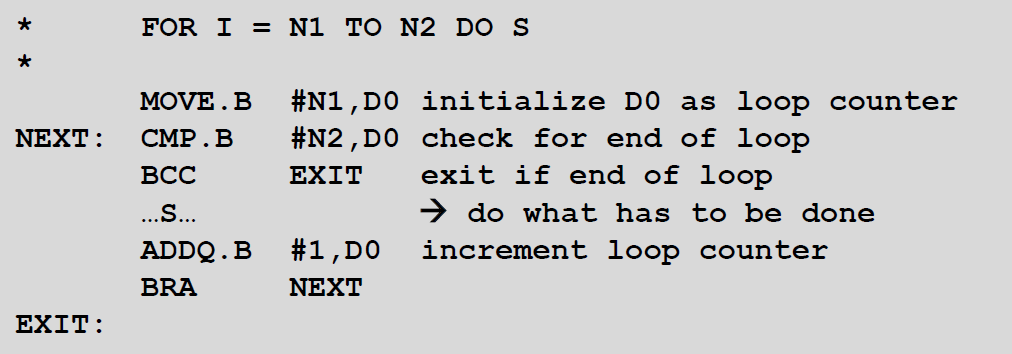
\includegraphics[width=9cm]{images/For.PNG} & \raisebox{0.9cm}{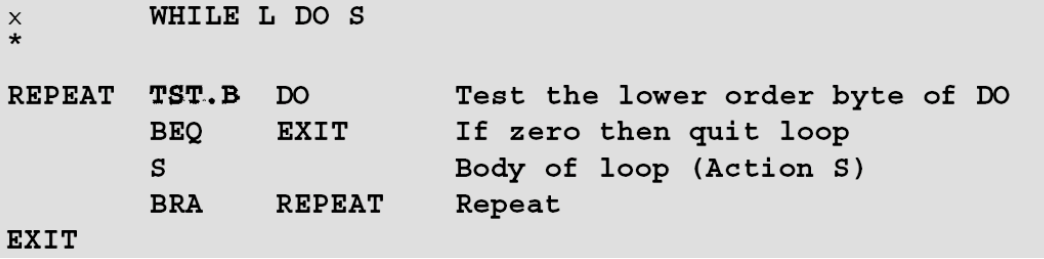
\includegraphics[width=9cm]{images/While.PNG}} \\
	\hline
	\textbf{case I of I1:S1, I2:S2 ,\ldots , default:Sd} & \textbf{repeat S until L} \\
  	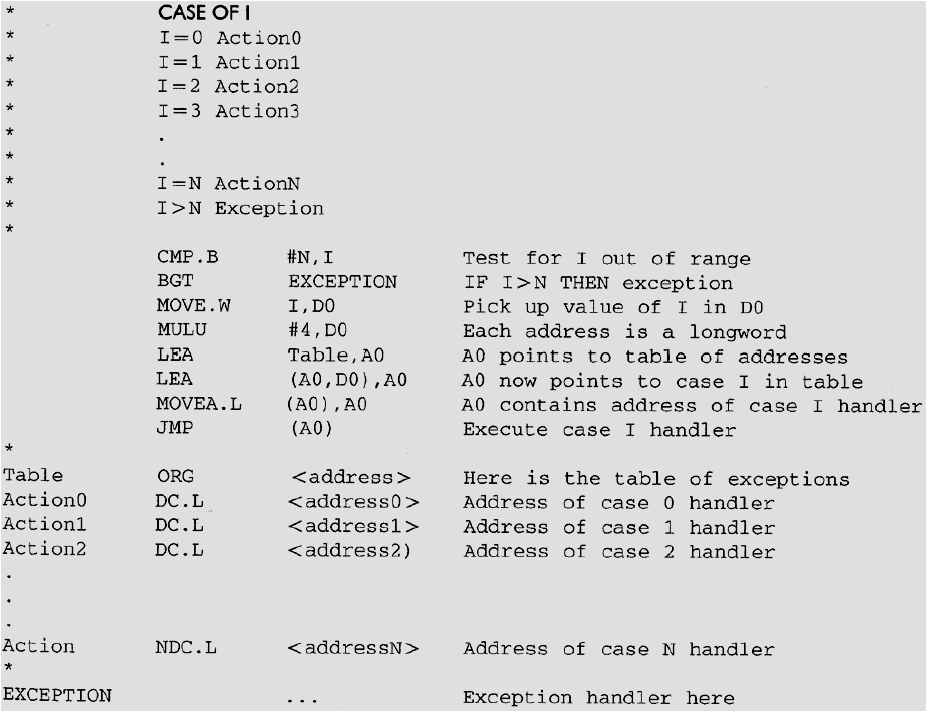
\includegraphics[width=9cm]{images/Case.PNG} & \raisebox{4.9cm}{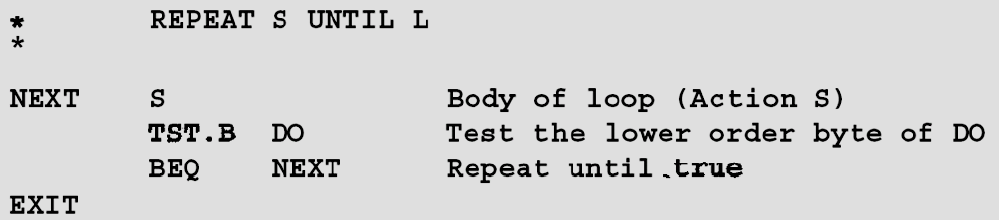
\includegraphics[width=9cm]{images/Repeat.PNG}} \\
	\hline
\end{tabular}
